\documentclass{article}
\usepackage{animate}
\usepackage{listings}
\usepackage{float}
% Language setting
% Replace `english' with e.g. `spanish' to change the document language
\usepackage[english]{babel}
% Set page size and margins
% Replace `letterpaper' with `a4paper' for UK/EU standard size
\usepackage[letterpaper,top=2cm,bottom=2cm,left=3cm,right=3cm,marginparwidth=1.75cm]{geometry}

% Useful packages
\usepackage{amsmath}
\usepackage{graphicx}
\usepackage[colorlinks=true, allcolors=blue]{hyperref}

\title{HAMS1K: Hardware Accelerated Merge Sort for sorting array of 1024 integers}
\author{Gaurav Dubey, Michael Salek}

\begin{document}
\maketitle

\begin{abstract}
This paper, presents HAMS1K, a very basic hardware accelerated sorting algorithm designed to sort a 1024 integer input array. HAMS1K utilizes Amdhal's Law to speedup the performance of a sort function. By running on Hardware certain tasking can be run in parallel to increase the actions completed per clock cycle. The implemented algorithm divides an unsorted array of 1024 integers into 256 sublists of 4 integers each. These 256 sublists are then sorted using a bitonic sort hardware implementation. Later hardware employs a parallel merge tree to repeatedly merge sublists until only one sublist remains. This sublist corresponds to the desired sorted list. This hardware implementation can only sort 1024 integers in its current form, but with some changes and a supporting application software, any unsorted array can be sorted. 
\end{abstract}

\section{Introduction}

Sorting is used in a variety of applications that deal with large amounts of data. Computers are processing more data than ever before thanks to cloud computing, machine learning, artificial intelligence, and the internet of things. As Moore's law slows, there is concern that the increase in compute resources will not be enough to meet the demand for compute resources to handle data that grows exponentially every year.

Sorting data involves subtasks such as comparing and swapping two integers. A function to swap two integers in C/C++ can be written in as few as four assignment statements, as shown below, but this does not imply that the computer will execute this function in four machine instructions after the code is compiled and converted to machine code. Looking at the disassembled code of the swap function below, it can be seen that the C/C++ compiler added a few more instructions to allow the machine to produce the desired results. These additional inserted instructions are required and consume a substantial number of compute time. In addition, there may be cases where the swap function is called for a variable involving cache misses, which will increase the execution time even more. 


\begin{lstlisting}
C/C++ code:
void swap(int * i, int *j) {
  int a = *i;   int b = *j;
  *i = b;       *j = a;
}

assembly:
    pushl %ebp          #setup, push data on stack for swap
    movl  %esp,%ebp     #setup
    pushl %ebx          #setup, push data on stack for swap
    movl  8(%ebp),%edx  #edx = i
    movl  12(%ebp),%ecx #ecx = j
    movl  (%edx),%ebx   #ebx = *i
    movl  (%ecx),%eax   #ecx = *j
    movl  %eax,(%edx)   #*i = b
    movl  %ebx,(%ecx)   #*j = a
    popl  %ebx          #finish, remove data from stack
    popl  %ebp          #finish, remove data from stack
    ret                 #finish
\end{lstlisting}

As shown, basic operations like swap which seem trivial could be quite more expensive than expected, and sorting large amounts of data consumes significant compute resources. Dedicated hardware for this problem can swap two variables in just 1 machine cycle. Due to this, there is a growing interest in reducing the time required to perform a function by designing application-specific solutions to accelerate sorting algorithms in hardware. HAMS1K is one such attempt to speed up merge sorting through parallelism and locality.

HAMS1K includes RAMs to store data locally to avoid large memory read and write accesses latency. The hardware implementation consists of multiple RAMs where read and write accesses are performed in a manner that parallel merge tree can operate at optimal rates to speed up sorting. 


\section{Background}
A computer must be able to perform multiple compare and swap operations in a single machine cycle in order to sort data at high throughput. The complexity of designing computing systems that can perform multiple operations simultaneously and have memory elements to accommodate required data is a major barrier to achieving this. There are networks with fast sorting or ordering capabilities, such as the Batcher odd-even mergesort network, the Bitonic merge sorter network, and the FIFO-based Merge Sorting network, among others. HAMS1K speeds up the merge sort algorithm by utilising a bitonic merge sort network and a FIFO-based merge network.  

\subsection{Amdahl's Law}
In computer architecture, Amdahl's law (or Amdahl's argument) is a formula which gives the theoretical speedup in latency of the execution of a task at fixed workload that can be expected of a system whose resources are improved. Amdahl's Law can be utilized across many functions to implement parallelism thus improving the speed at which functions can be performed. The expected Speedup by implementing this can be found by the following equation:

\[Speedup = \frac{\text{Execution time without enhancement}}{\text{Execution time with enhancement}} = \frac{1}{(1-f)+f/n} \]

where f = fraction of program that is parallelizable and n = parallel processors. This assumes that the parallelizable work distributes perfectly onto n processors of equal capability.

\subsection{Merge Sort}
Merge Sort is a Divide and Conquer algorithm. Implementation of this algorithm involves three steps i.e. divide, conquer and merge. The algorithm divides the input array into two sublists, then it separates these two sublists into four sublists, this process is continued until the lists are broken down until they can no longer be divided, leaving N sublists with just 1 element each, these N sublists can be considered as sorted. Here N is the length of the input array to be sorted.
Once these lists cannot be broken down further, it starts merging these N sublists such that merged lists are sorted in a particular order (say ascending order), conquering sort problem one step at a time. This process is illustrated with animation in the figure \ref{fig:merge_serial}.

\begin{figure}[H]
\centering
  \animategraphics[loop,controls,width=\linewidth]{1}{merge_sort_animation/Slide}{1}{9}
\caption{\label{fig:merge_serial}Illustration of the Merge sort algorithm.}
\end{figure}

\subsection{Batcher odd–even mergesort}
\label{subsec:Batcher odd–even mergesort}
Batcher's odd–even mergesort is a generic construction devised by Ken Batcher for sorting networks of size $O(nlog^2n)$ and depth $O(nlog^2n)$, where n is the number of items to be sorted\cite{wiki:001}\cite{art1}. Although it is not asymptotically optimal, Knuth concluded in 1998, with respect to the AKS network that "Batcher's method is much better, unless n exceeds the total memory capacity of all computers on earth!"

It is popularized by the second GPU Gems book, as an easy way of doing reasonably efficient sorts on graphics-processing hardware.

\begin{lstlisting}
Pseudo code:

# note: the input sequence is indexed from 0 to (n-1)
for p = 1, 2, 4, 8, ... # as long as p < n
  for k = p, p/2, p/4, p/8, ... # as long as k >= 1
    for j = mod(k,p) to (n-1-k) with a step size of 2k
      for i = 0 to k-1 with a step size of 1
        if floor((i+j) / (p*2)) == floor((i+j+k) / (p*2))
          compare and sort elements (i+j) and (i+j+k)
\end{lstlisting}

\begin{figure}[H]
\centering
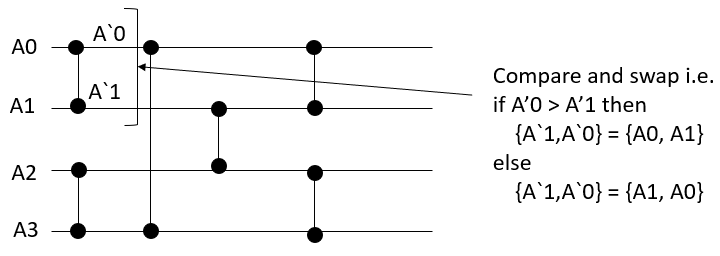
\includegraphics[width=1.00\textwidth]{odd_even_nwk.PNG}
\caption{\label{fig:odd_even_nwk}A hardware oriented design to sort list of 4 elements (Batcher odd–even mergesort).}
\end{figure}

\subsection{Bitonic Mergesort}
\label{subsec:Bitonic Mergesort}


Bitonic mergesort is a parallel algorithm for sorting\cite{wiki:002}. It is also used as a construction method for building a sorting network. The algorithm was devised by Ken Batcher. The resulting sorting networks consist of  $O(nlog^2(n))$ comparators and have a delay of $O(nlog^2n)$, where $n$ is the number of items to be sorted.

\begin{lstlisting}
Pseudo code:
// given an array arr of length n, this code sorts it in place
// all indices run from 0 to n-1
for (k = 2; k <= n; k *= 2) // k is doubled every iteration
  // j is halved at every iteration, with truncation of fractional parts
  for (j = k/2; j > 0; j /= 2) 
    for (i = 0; i < n; i++)
      l = bitwiseXOR (i, j); // in C-like languages this is "i ^ j"
      if (l > i)
        if ((bitwiseAND (i, k) == 0) AND (arr[i] > arr[l])
          OR (bitwiseAND (i, k) != 0) AND (arr[i] < arr[l]) )
           swap the elements arr[i] and arr[l]
\end{lstlisting}

\begin{figure}[H]
\centering
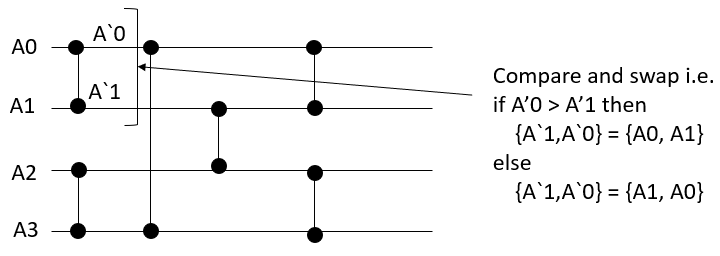
\includegraphics[width=1.00\textwidth]{bitonic_nwk.PNG}
\caption{\label{fig:bitonic_nwk}A hardware oriented design to sort list of 4 elements (Bitonic mergesort).}
\end{figure}

\subsection{FIFO-based Merge Sort}
\label{subsec:FIFO-based Merge Sort}

The serial merge sort algorithm can be implemented in hardware by using a network (FIFO merge) of circular buffers, as shown in figure \ref{fig:fifo_nwk}. Because the algorithm divides the input array first, an array with N elements will have N sorted sublists. We use the FIFO merge to combine sorted N sublists into N/2 sorted lists with 2 elements. Then we combine N/2 sorted lists to make N/4 sorted lists, each with four elements. This process is repeated until we have a list of N elements.


\begin{figure}[H]
\centering
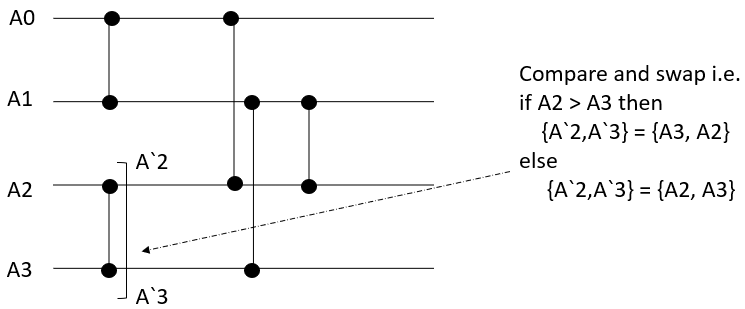
\includegraphics[width=1.00\textwidth]{fifo_nwk.PNG}
\caption{\label{fig:fifo_nwk}A hardware oriented design to merge two sorted list using FIFO-base merge.}
\end{figure}



\section{Hardware accelerated Merge Sort implementations}
\subsection{Implementation I: serial implementation}
\label{subsec:Implementation I}
A serial merge sort implementation can be designed using RAM to store the input array to be sorted and a FIFO-based merge sorter. A finite state machine would generate addresses for read and write access for compare and swap operations in this case. The FIFO-based merge sorter, as discussed in section~\ref{subsec:FIFO-based Merge Sort}, performs compare and swap operations.

Assuming that RAM does not support simultaneous read and write, the hardware implementation will take 2N*$(log_2N-1)$ clock cycles to sort the input array. Because the merging process is repeated $log_2N-1$ times, each merging cycle requires N clock cycles to read all array elements and N clock cycles to write the merged sorted list back to memory.

An illustration of this implementation that sorts an array of 12 elements is shown with animation in figure~\ref{fig:address_serial}.

\begin{figure}[H]
\centering
  \animategraphics[loop,controls,width=\linewidth]{1}{address_serial}{1}{33}
\caption{\label{fig:address_serial}Illustration of hardware implementation of serial Merge sort algorithm.}
\end{figure}


\subsection{Implementation II: serial hybrid implementation}
\label{subsec:Implementation II}
Odd-even sorter and bitonic sorter can sort a list of elements of power of 2 at a time, as discussed in sections~\ref{subsec:Batcher odd–even mergesort} and~\ref{subsec:Bitonic Mergesort}, odd-even sorter and bitonic sorter can sort a list of elements of power of 2 at a time. While a FIFO-based merge sorter can sort multiple lists at the same time, the output rate is always one number per clock cycle. This implementation uses these networks for the initial sorting to increase throughput and a FIFO-based sorter for the rest of the sorting.
 
In the case of the implementation discussed in section ~\ref{subsec:Implementation I}, merge sorting begins with merging lists with one element, then lists with two elements, lists with four elements, and so on. Because hardware can now sort lists with $2^M$ elements, the first M merge cycles can be avoided by using a $2^M$ element bitonic sorter for initial sorting. 

Assuming that RAM does not support simultaneous read and write, the hardware implementation will take 2N*$(log_2N-M+1)$ clock cycles to sort the input array. Because the merging process is repeated $log_2N-M-1$ times (including the first merge cycle by bitonic sort), each merging cycle requires N clock cycles to read all array elements and N clock cycles to write the merged sorted list back to memory.

An illustration of first merge sort cycle by bitonic sorter is shown with animation in figure~\ref{fig:serial}.

\begin{figure}
\centering
  \animategraphics[loop,controls,width=\linewidth]{1}{ad-}{1}{8}

\caption{\label{fig:serial}Initial merge cycle using bitonic sorter for ~\ref{subsec:Implementation II}.}
\end{figure}


\subsection{Implementation III: improved hybrid implementation}
\label{subsec:Implementation III}

In section ~\ref{subsec:Implementation II} the hybrid implementation needs a deserailizer unit which concatenates $2^M$ elements i.e. to prepare input data for $2^M$ bitonic sorter. By use of multiple RAMs which could support reads and write of $2^M$ integers per clock as shown with animation in figure~\ref{fig:impl3}, deserailizer could be avoided, also reading and writing all array element could be done in $N/2^M$ clock cycles instead of N clock cycles for merge cycles. Additionally, number of merge cycle also reduce to $log_MN-1$ from $log_2N-1$.

HAMS1K is based on the this improved hybrid implementation. This implementation required hardware architecture changes to improve parallelism. The architecture of HAMS1K is shown in figure ~\ref{fig:scheme}.

Assuming that RAM does not support simultaneous read and write, the hardware implementation will take $N*(log_MN)+(N/2^M)*(log_MN)$ clock cycles to sort the input array. Because the merging process is repeated $log_2N-M$ times (excluding the first merge cycle by bitonic sort), each merging cycle requires $N/2^M$ clock cycles to read all array elements and N clock cycles to write the merged sorted list back to memory.
\begin{figure}[H]
\centering
  \animategraphics[loop,controls,width=0.90\textwidth]{1}{impl3_animation/Slide}{1}{19}
\caption{\label{fig:impl3}Illustration of improved hybrid implementation.}
\end{figure}

\begin{figure}[H]
\centering
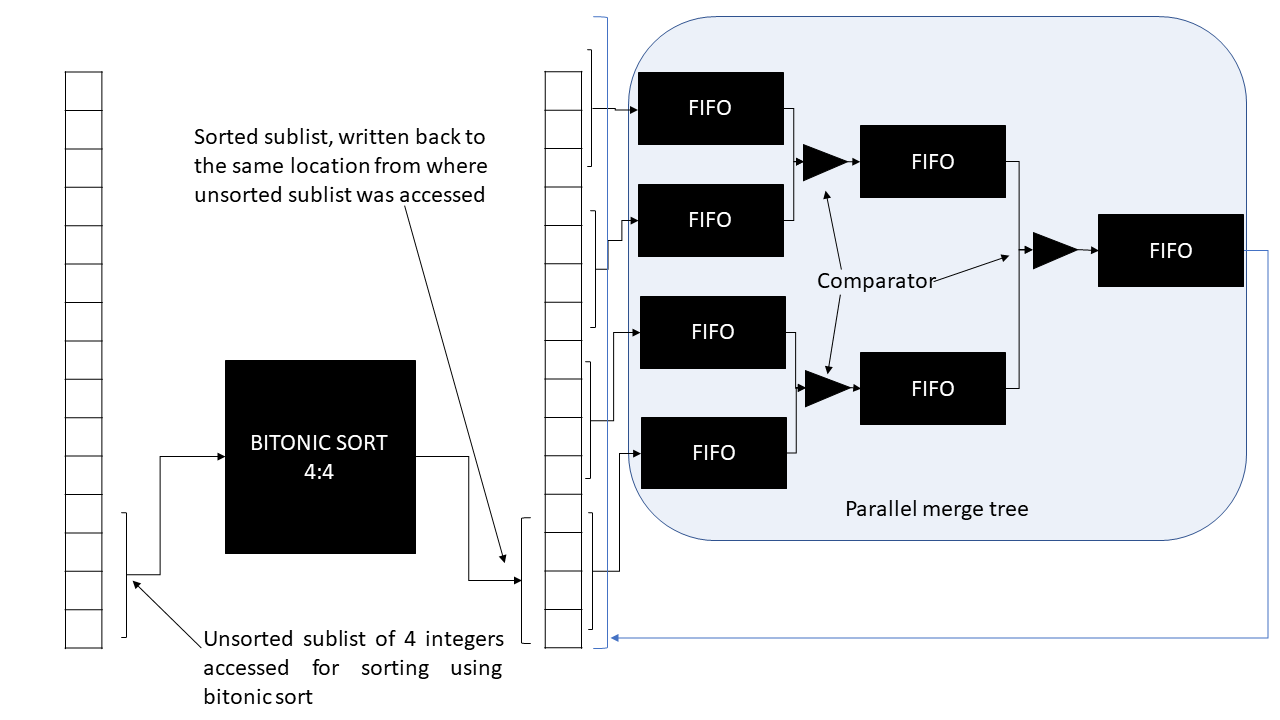
\includegraphics[width=0.90\textwidth]{hams_scheme.png}
\caption{\label{fig:scheme}Block diagram of HAMS1K hardware.}
\end{figure}


\section{Results and conclusion}

Various hardware architecture have been tested for performance and it is observed that parallelism plays a major factor in reduction of the execution time for sorting.  --- see Table~\ref{tab:widgets}. Also, increasing width of bitonic sorter and odd-even sorter is desirable to increase parallelism but this increases overall area of the design and complexity in handling memory interface for merge sort. With  increase in parallelism, sorting rate improves proportionally but at cost of area and complexity.
Deciding optimal degree of parallelism is beyond the scope of this work.

All test have been performed for hardware designed to sort 1024 integers and the width of bitonic sorter network and FIFO-based merge sorter is four for ~\ref{subsec:Implementation II} and ~\ref{subsec:Implementation III}. 
\begin{table}[H]
\centering
\begin{tabular}{l|c|c}
Hardware implementation (1024 element sorter) & Computation time in clock cycles & SpeedUp \\\hline
Implementation I & 18432 & 1.0\\
Implementation II & 14336 & 1.3\\
Implementation III (HAMS1K) & 5384 & 3.4
\end{tabular}
\caption{\label{tab:widgets}Computation time in terms of clock cycles for various hardware implementations.}
\end{table}

\bibliographystyle{alpha}
\bibliography{references}

\end{document}